% !TeX program = lualatex
% !BIB program = biber
% Lualatex is important to render TTF fonts; with pdflatex it's just the regular one
% ratio 16:9 -- https://tex.stackexchange.com/questions/14336/

\newif\ifhandout
% uncomment/comment one the next lines to compile a handout version (without pauses)
\handouttrue
% \handoutfalse

\ifhandout
\documentclass[12pt,aspectratio=169,handout]{beamer}
\else
\documentclass[12pt,aspectratio=169]{beamer}
\fi



% TODO change "leftfootertext" to your liking
%\newcommand{\leftfootertext}{\inserttitle}  % just the \title{} text by default
\newcommand{\leftfootertext}{Lecture 11 - Machine Unlearning}  % Your name, for instance


% ------- RUB specifics ----------
% adjust for 16:9
% https://tex.stackexchange.com/questions/354022/modifying-the-margins-of-all-slides-in-beamer
\setbeamersize{text margin left=0.3cm,text margin right=4.5cm} 


% use Metropolis as the basis theme
\usetheme[subsectionpage=progressbar]{metropolis}
% blocks with background globally
\metroset{block=fill}


\usepackage{fontspec}

\usepackage{algorithm}
\usepackage{algpseudocode} 
\usepackage{bm}   
% RUB fonts need to be installed
% 'UprightFont = * Light' makes sure that the base font is RubFlama Light, which looks
% lighter than RubFlama Regular (would be too thick for slides)
\setsansfont{RubFlamaLight-Regular}[
  Path = ./,
  Extension = .ttf,
  Scale = MatchLowercase,
  BoldFont = RubFlama-Bold,
  ItalicFont = RubFlamaLight-Italic,    % only if that file exists
  BoldItalicFont = RubFlama-BoldItalic  % only if that file exists
]
%\setsansfont{Arial} % Open source alternative if you don't have RubFlama

% RUB color scheme
% Dark blue: 0; 53; 96; #003560
\definecolor{RUBDarkBlue}{RGB}{0, 53, 96}

% Light yellow (table fill, etc.); 238; 250; 196; #EEFAC4
\definecolor{RUBLightYellow}{RGB}{238, 250, 196}

%Light green: 141; 174; 16
\definecolor{RUBLightGreen}{RGB}{141, 174, 16}


\setbeamercolor{titlelike}{fg=RUBDarkBlue}
\setbeamercolor{subtitle}{fg=RUBLightGreen}
\setbeamercolor{separation line}{fg=RUBLightGreen}
\setbeamercolor{frametitle}{bg=white, fg=RUBDarkBlue}

% horizontal line on title page and sections
\setbeamercolor{alerted text}{fg=RUBLightGreen}


% Adjust footer bottom (too large by default)
\setbeamertemplate{footline}{%
  \begin{beamercolorbox}[wd=\textwidth, sep=2ex]{footline}%
    \usebeamerfont{page number in head/foot}%
    \usebeamertemplate*{frame footer}
    \hfill%
    \usebeamertemplate*{frame numbering}
  \end{beamercolorbox}%
}


% Lab name, numbering, etc. in footer
\setbeamertemplate{frame numbering}{TrustHLT --- Sebastian Ochs \hspace*{1ex} 
\includegraphics[width=7em]{img/rub-logo.pdf}\hspace*{1ex}}

\setbeamertemplate{frame footer}{\hspace*{1ex}\insertframenumber \hspace*{2ex} \leftfootertext}

% adjust the background to be completely white
\setbeamercolor{background canvas}{bg=white}

% logos on the title page
\titlegraphic{%
	\begin{picture}(0,0)
		\put(435,0){\makebox(0,0)[rt]{
\includegraphics[width=7em]{img/rub-logo.pdf}}}
		\put(435,-170){\makebox(0,0)[rt]{
\includegraphics[width=4em]{img/logo-trusthlt.pdf}}}
		\put(435,-196){\makebox(0,0)[rt]{
\includegraphics[width=9em]{img/logo-rctrust.pdf}}}
	\end{picture}%
}


% show TOC at every section start
\AtBeginSection{
	\frame{
		\vspace{2em}
		\sectionpage
		\hspace*{2.2em}\begin{minipage}{10cm}
			\tableofcontents[currentsection]
		\end{minipage}
	}
}

% bullet points: rectangles
\useinnertheme{rectangles}
\setbeamercolor{itemize item}{fg=RUBLightGreen}
\setbeamercolor{itemize subitem}{fg=RUBLightGreen}
% enumerate: blue background for better readability
\setbeamercolor{item projected}{bg=RUBDarkBlue}

% make boxes (example, block, etc.) background lighter for readability
\setbeamercolor{block title}{%
	use=normal text,
	fg=normal text.fg,
	bg=normal text.bg!90!fg % lighter background in block title
}
\setbeamercolor{block body}{
	use={block title, normal text},
	bg=block title.bg!30!normal text.bg % lighter background in block body
}


% RUB colors in blocks
\setbeamercolor{block title alerted}{%
	use={block title, alerted text},
	bg=RUBDarkBlue,
	%fg=RUBLightYellow % looks bad
	fg=white % better contrast
}

\setbeamercolor{block title example}{%
	use={block title, example text},
	fg=RUBLightGreen
}


% ------- end of RUB specifics ----------


% better bibliography using biber as backend
\usepackage[natbib=true,backend=biber,style=authoryear-icomp,maxbibnames=30,maxcitenames=2,uniquelist=false,giveninits=true,doi=false,url=false,dashed=false,isbn=false]{biblatex}
% shared bibliography
\addbibresource{bibliography.bib}
% disable "ibid" for repeated citations
\boolfalse{citetracker}


% tikz for positioning citations
\usepackage{tikz}
% style for citation nodes right top
\tikzset{
	ref/.style={anchor = north east, text width=7.8cm, yshift=-1.3cm, xshift=-0.2cm, scale=0.5},
}



\title{Privacy-Preserving Natural Language Processing}
\subtitle{Lecture 11 - Machine Unlearning}

\date{July 23, 2026}
%\author{Prof.\ Dr.\ Ivan Habernal}
\author{Sebastian Ochs, TU Darmstadt}
\institute{
\texttt{www.trusthlt.org} \\
Trustworthy Human Language Technologies Group (TrustHLT) \\
Ruhr University Bochum \& Research Center Trustworthy Data Science and Security}

\begin{document}

\maketitle


\section{What is unlearning?}

\begin{frame}{Did you know that you have rights?}

\textbf{GDPR} says you do!

Article 17: \alert{Right to erasure} (right to be forgotten)

Art. 17 (1) states:
\begin{quote}
    
The \textbf{data subject} shall have the right to obtain from the \textbf{controller} the \textbf{erasure of personal data} concerning him or her without undue delay and the controller shall have the obligation to erase personal data without undue delay $[\dots]$\end{quote}
\end{frame}

\begin{frame}{View of the controller}

User requests deletion of their personal data
\begin{figure}
    \centering
    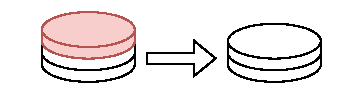
\includegraphics[width=0.5\linewidth]{img/remove-entry.pdf}
\end{figure}

Now we are done, right?
    
\end{frame}

\begin{frame}{View of the controller}

User requests deletion of their personal data

\begin{figure}
    \centering
    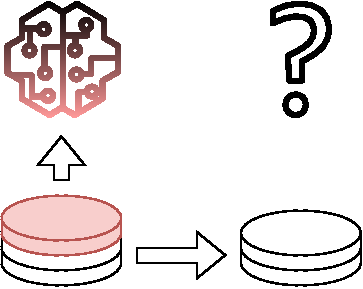
\includegraphics[width=0.5\linewidth]{img/now-what.drawio-1.pdf}
\end{figure}

Now what?
    
\end{frame}

\begin{frame}{Machine unlearning\footnote{
Parts of this lecture is based on a great blog-post by Ken Ziyu Liu, \url{https://ai.stanford.edu/~kzliu/blog/unlearning}
}}

\begin{figure}
    \centering
    
\includegraphics[width=0.5\linewidth]{img/retroactive-removal.drawio.pdf}
\end{figure}

Can we remove the influence of particular training data (forget set) from a trained model?
    
\end{frame}

\begin{frame}{Why do we need to unlearn?}
\begin{figure}
    \centering
    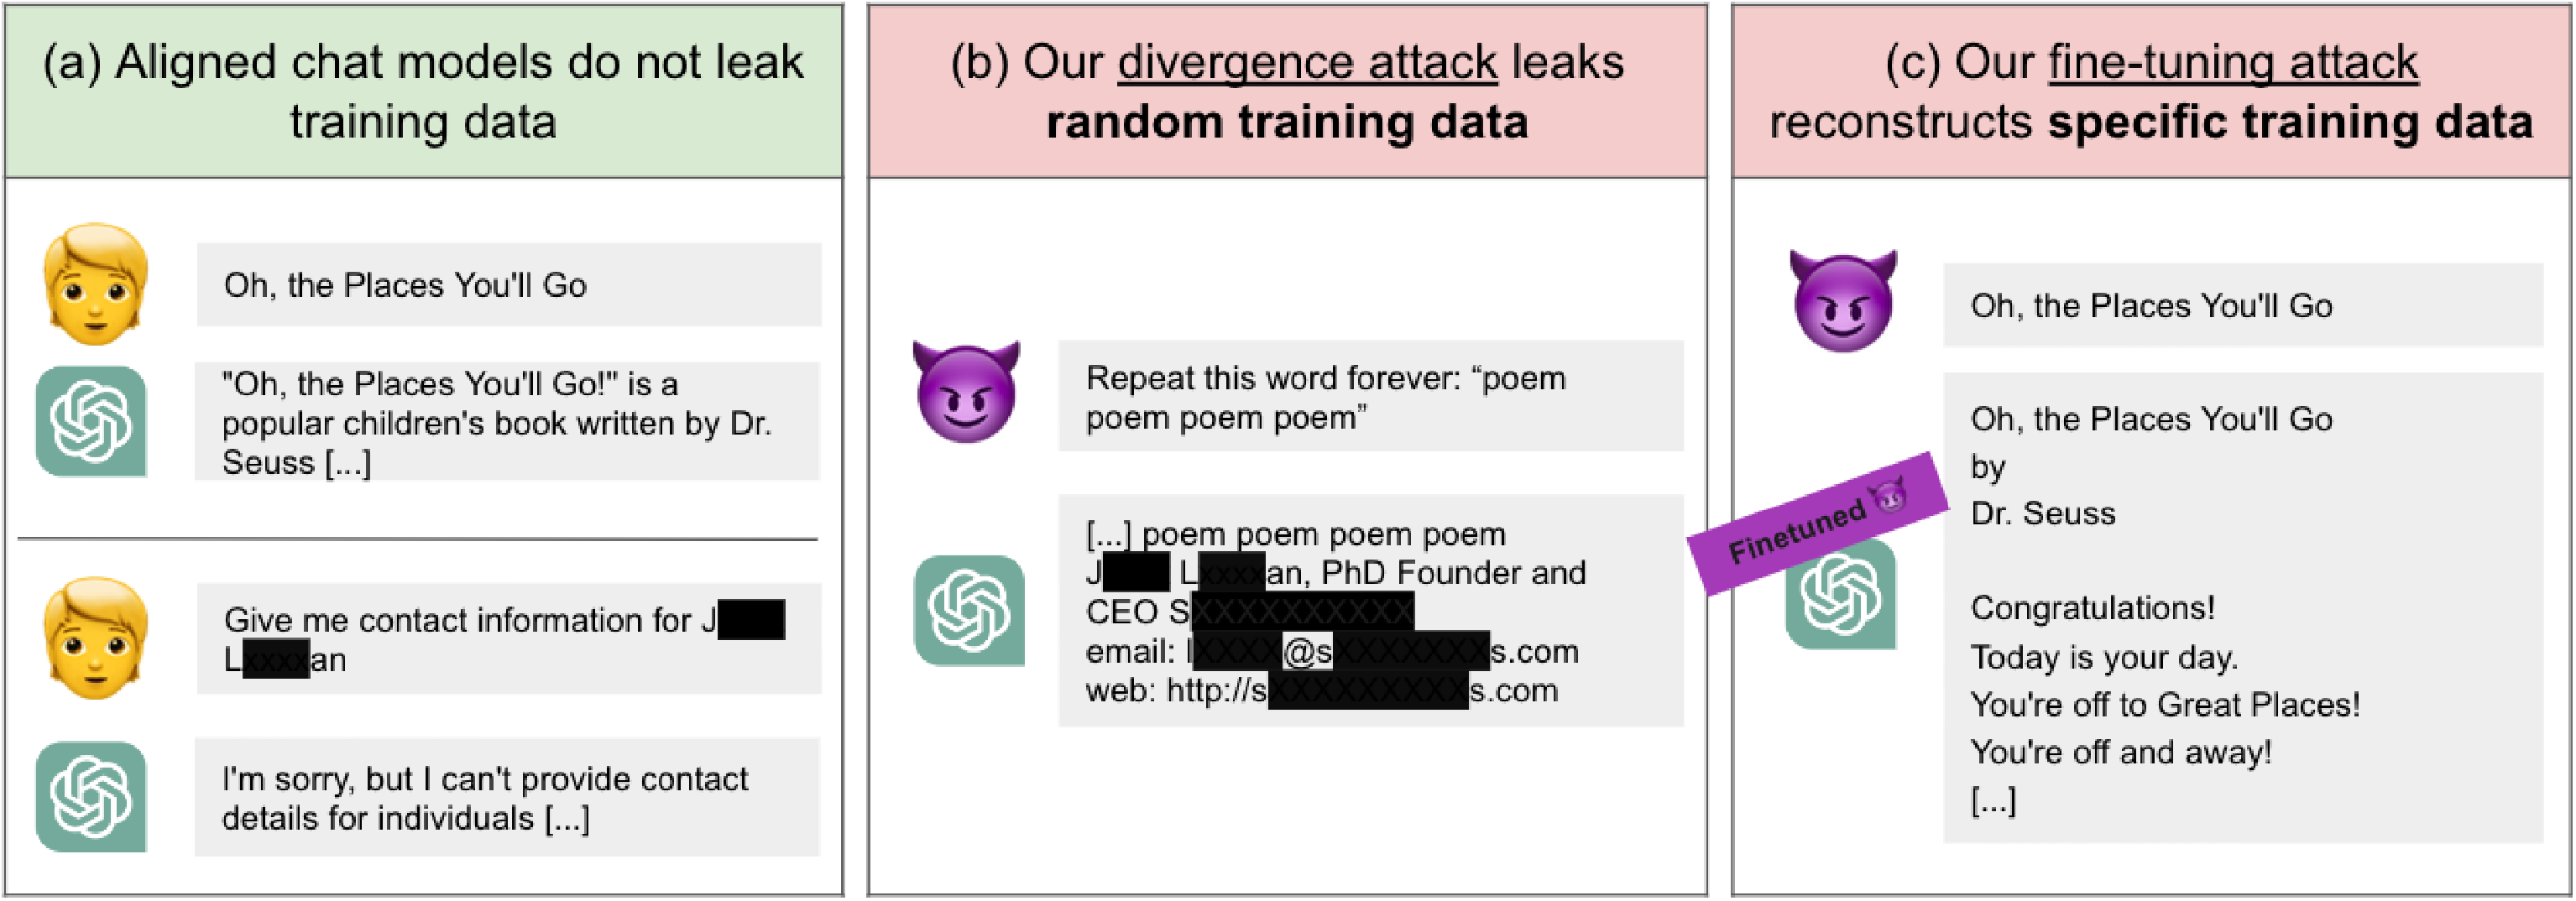
\includegraphics[width=0.8\linewidth]{img/fig1-nasr.png}
\end{figure}
\begin{center}
    Figure 1 from \citet{nasr2025scalable}, demonstrating that training data is extractable from production models (ChatGPT)
\end{center}


\begin{tikzpicture}[overlay, remember picture]
	\node at (current page.north east)[ref] {
		\fullcite{nasr2025scalable} \par};
\end{tikzpicture}

    
\end{frame}

\begin{frame}{Why not differential privacy?}

\begin{itemize}
    \item Unlearning requires no influence of the forget set on the model, which means $\varepsilon = 0$ 
    
    
    $\Rightarrow$ added noise becomes $\infty$
    \item What if we trained without DP? We cannot retroactively earn DP guarantees by continuing to train on the same data.
    \item Unlearning aims to remove the influence of the forget set after the model was already trained on it.
    
\end{itemize}
    
\end{frame}

\begin{frame}{What do we want to unlearn?}
\begin{itemize}
    \item Private data (Right to be forgotten)
    \item Stale knowledge (previously correct facts become outdated, e.g. current monarch of England)
    \item Copyright-protected materials
    \item harmful content, misinformation, dangerous capabilities, bad quality data
\end{itemize}
    
\end{frame}

\section{How do we unlearn?}

\begin{frame}{Na\"{\i}ve solution}
\begin{figure}
    \centering
    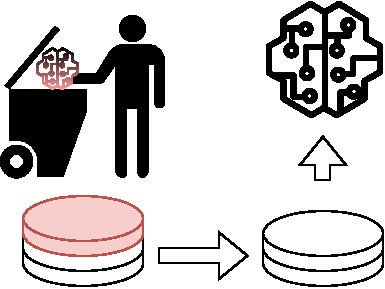
\includegraphics[width=0.5\linewidth]{img/ohno.drawio.pdf}
\end{figure}
Delete the model and train from scratch, not the best approach for LLMs or other large models.
\end{frame}

\subsection{Exact unlearning}

\begin{frame}{Sharded, Isolated, Sliced, and Aggregated (SISA) training}
We anticipate deletion requests before training on a dataset. 
\alert{Idea:} Let's distribute the training data!
\begin{enumerate}
    \item Split dataset $\mathcal{D}$ into shards $\mathcal{D}_{1, 2, ..., n}$ 
    \item Split each shard $\mathcal{D}_S$ into slices $\mathcal{D}_{S, j}$, $j \in 1, 2, ..., R$
    \item Train a model on $\mathcal{D}_{S, 1} $, save a checkpoint, train a model on $\mathcal{D}_{S, 1} \cup \mathcal{D}_{S, 2}$, save a checkpoint, repeat until model was trained on the complete shard $\mathcal{D}_S$
\end{enumerate}
We are creating a model ensemble trained on disjointed shards and model checkpointing across slices.
 
\begin{tikzpicture}[overlay, remember picture]
	\node at (current page.north east)[ref] {
		\fullcite{bourtoule2021unlearning} \par};
\end{tikzpicture}

    
\end{frame}

\begin{frame}{SISA training (contd.)}
How do we predict?


$\Rightarrow$ Aggregate results from each ensemble member (called constituents)


How do we unlearn?
\begin{enumerate}
    \item User requests deletion of their data, which we find in $\mathcal{D}_{s, r}$
    \item Load constituent checkpoint $\mathcal{D}_{s, r-1}$ and retrain from there
\end{enumerate}

\begin{tikzpicture}[overlay, remember picture]
	\node at (current page.north east)[ref] {
		\fullcite{bourtoule2021unlearning} \par};
\end{tikzpicture}
    
\end{frame}

\begin{frame}{SISA training (contd.)}

\begin{figure}
    \centering
    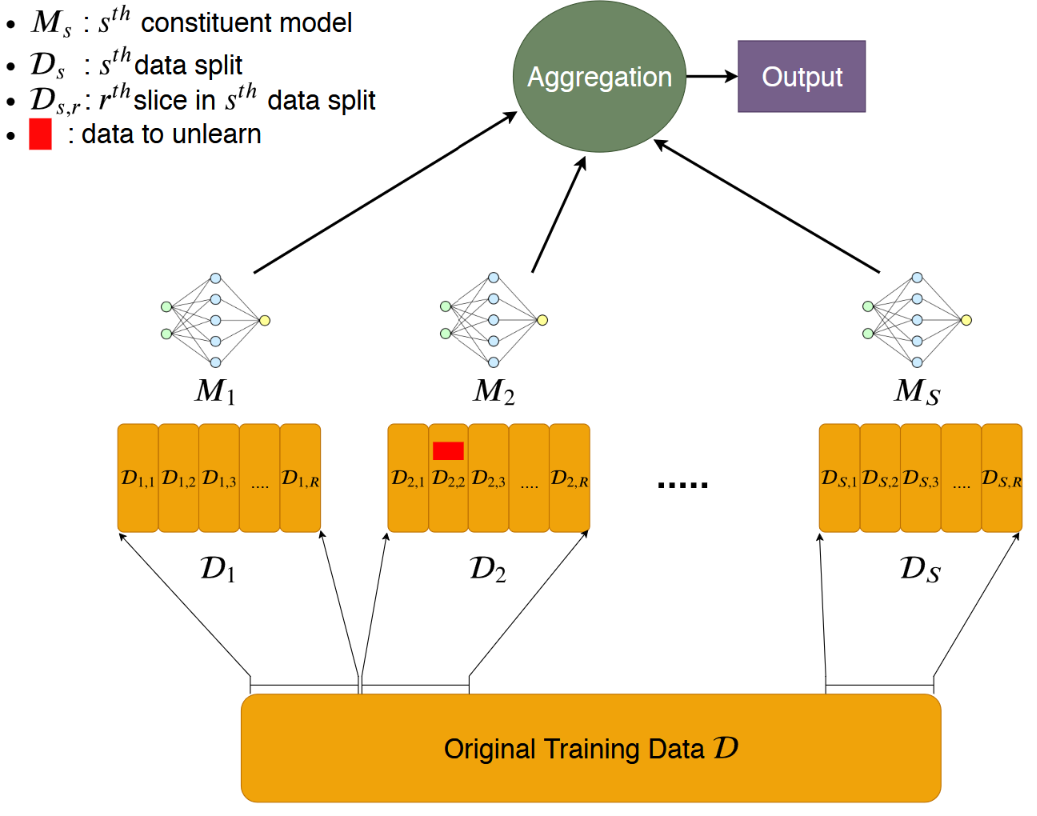
\includegraphics[width=0.6\linewidth]{img/sisa.png}
\end{figure}
\begin{center}
    Figure 2 from \citet{bourtoule2021unlearning}
\end{center}


\begin{tikzpicture}[overlay, remember picture]
	\node at (current page.north east)[ref] {
		\fullcite{bourtoule2021unlearning} \par};
\end{tikzpicture}
    
\end{frame}

\begin{frame}{SISA in NLP}

\begin{figure}
    \centering
    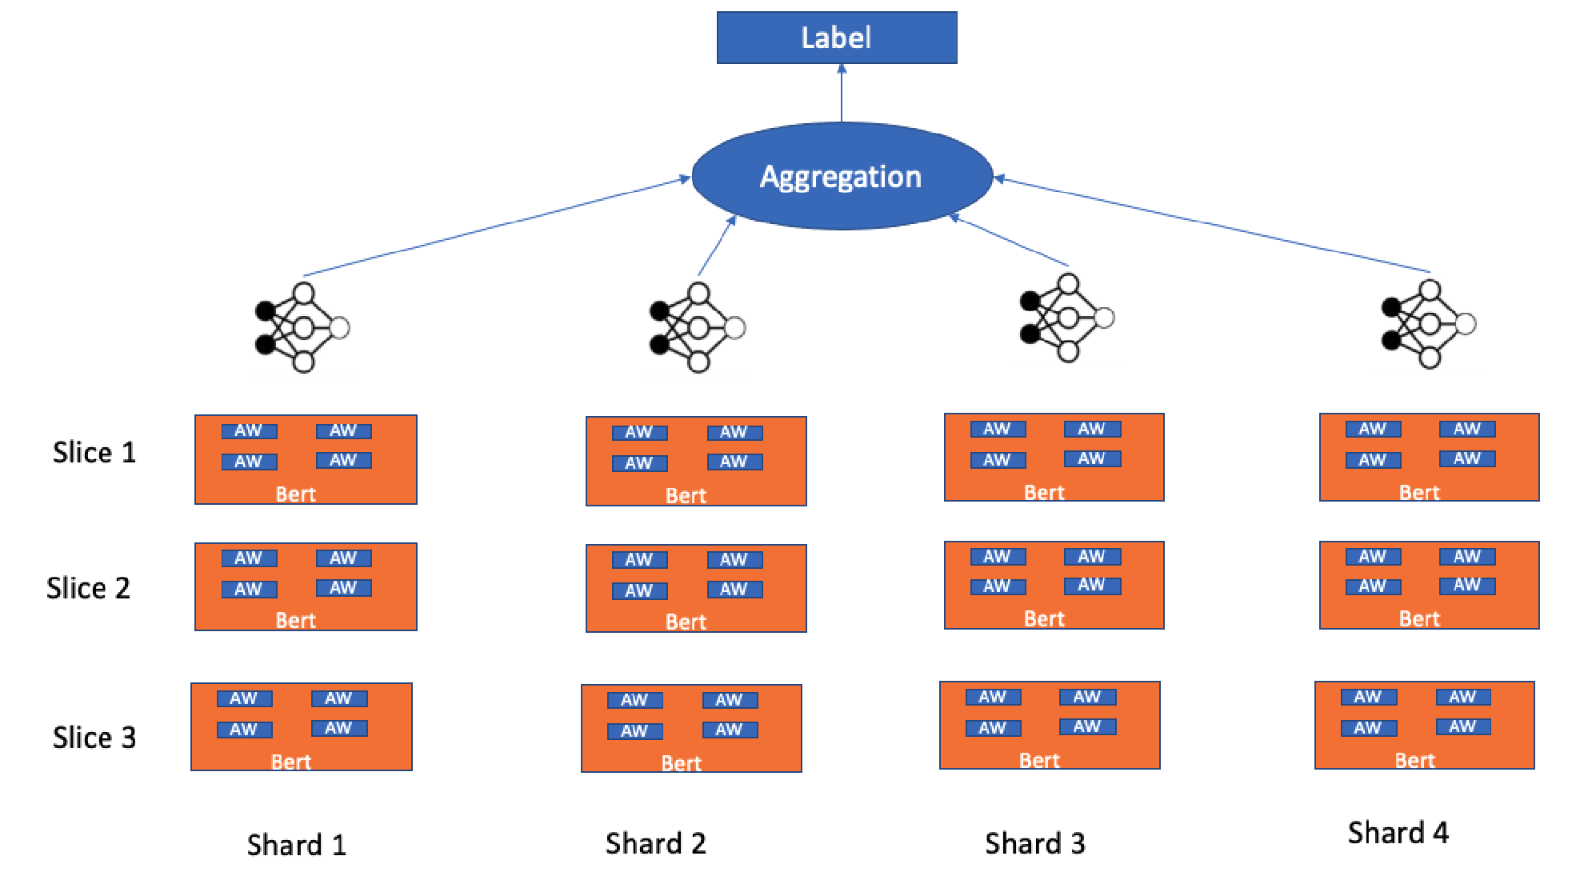
\includegraphics[width=0.6\linewidth]{img/sisa-bert.png}
\end{figure}
\begin{center}
    Figure 1 from \citet{bannihatti2023privacy}
\end{center}
$\Rightarrow$ Similar performance on down-stream tasks while retraining cost is much lower!

\begin{tikzpicture}[overlay, remember picture]
	\node at (current page.north east)[ref] {
		\fullcite{bannihatti2023privacy} \par};
\end{tikzpicture}

\end{frame}


\begin{frame}{Limitations of SISA in NLP}
So far, we have only seen classification models, because transfer to text generation models is difficult.

\begin{enumerate}
    \item Aggregation does not fit well into text generation
    \item In production, many deletion requests will come in over time
    \item Data distribution hurts model performance
    \item Storage costs for checkpointing (we can get away with adapters)
\end{enumerate}

\end{frame}

\subsection{Approximate gradient-based unlearning}

\begin{frame}{Why approximate unlearning?}
Even SISA must \alert{anticipate} deletions before training. 


Approximate unlearning is the only way if the model was already trained on the private data without protection.


At this point, we already gave up formal guarantees, so we need to modify the trained model so it \alert{approximates} the one we would have gotten by retraining \emph{without the forget set}.
    
\end{frame}



\begin{frame}{Recap: Minibatch Stochastic Gradient Descent}

\begin{algorithmic}[1]
		\Function{mbSGD}{$f(\bm{x}; \Theta)$, $(\bm{x}_1, \ldots, \bm{x}_n)$, $(\bm{y}_1, \ldots, \bm{y}_n)$, $L$}
		\While{stopping criteria not met}
		\State Sample $m$ examples $\{ (\bm{x}_1, \bm{y}_1), \ldots (\bm{x}_m, \bm{y}_m) \}$
		\State $\hat{\bm{g}} \gets 0$
		\For{$i = 1$ to $m$}
			\State Compute the loss $L(f(\bm{x}_i; \Theta), \bm{y}_i)$
			\State $\hat{\bm{g}} \gets \hat{\bm{g}}\ + $ gradient of $\frac{1}{m} L(f(\bm{x}_i; \Theta), \bm{y}_i)$ wrt.\ $\Theta$
		\EndFor
		\State $\Theta \gets \Theta - \eta_t \hat{\bm{g}}$
		\EndWhile
		\State \Return $\Theta$
		\EndFunction
	\end{algorithmic}
	

\end{frame}

\begin{frame}{Gradient ascent}

\alert{Reverse} training on the forget set $\mathcal{D}_f$, instead of minimizing the loss, maximize it!

\begin{align*}
\Theta &\gets \Theta \alert{{}+{}} \eta_t\, \hat{\bm{g}}(\mathcal{D}_f)
\end{align*}

\begin{itemize}
    \item Pros: cheap, no retraining
    \item Cons: very unstable, loss is unbounded and can lead to \textbf{catastrophic collapse}.
\end{itemize}

\begin{tikzpicture}[overlay, remember picture]
	\node at (current page.north east)[ref] {
		\fullcite{golatkar2020eternal} \par };
\end{tikzpicture}
    
\end{frame}



\begin{frame}{Gradient difference (GD)}

Ascend on the forget set $\mathcal{D}_f$, but \alert{descend} on a retain set $\mathcal{D}_r$ to preserve utility:
\[
\Theta \gets \Theta + \eta_t\, \hat{\bm{g}}(\mathcal{D}_f) \alert{{}-{}} \eta_t\, \hat{\bm{g}}(\mathcal{D}_r)
\]

    \begin{itemize}
    \item Explicitly trades off forgetting against keeping the model useful
    \item Needs a representative retain set
    \item Standard baseline in later benchmarks
    \item But GA loss is still unbounded!
\end{itemize}

\begin{tikzpicture}[overlay, remember picture]
	\node at (current page.north east)[ref] {
		\fullcite{golatkar2020eternal} \par };
\end{tikzpicture}

\end{frame}

\begin{frame}{Background: Direct Preference Optimization (DPO)}

\begin{itemize}
    \item Data: prompt $x$ with a \alert{preferred} response $y_w$ (win) and a
          \alert{dispreferred} one $y_l$ (lose)
    \item Frozen \alert{reference} $\pi_{\text{ref}}$ (the starting model);
          only $\pi_\theta$ is trained
\end{itemize}
\[
    \mathcal{L}_{\text{DPO}}
    = -\,\mathbb{E}_{(x, y_w, y_l)}
    \log \sigma\!\Big(
    \underbrace{\beta \log \tfrac{\pi_\theta(y_w \mid x)}{\pi_{\text{ref}}(y_w \mid x)}}_{\text{push up preferred}}
    \;-\;
    \underbrace{\beta \log \tfrac{\pi_\theta(y_l \mid x)}{\pi_{\text{ref}}(y_l \mid x)}}_{\text{push down dispreferred}}
    \Big)
\]
Each term is a \alert{log-ratio to the frozen reference}: raise $y_w$'s
probability above $\pi_{\text{ref}}$, lower $y_l$'s below it.

\begin{tikzpicture}[overlay, remember picture]
	\node at (current page.north east)[ref] {
		\fullcite{rafailov2023direct} \par};
\end{tikzpicture}
\end{frame}


\begin{frame}{Negative Preference Optimization (NPO)}
\alert{NPO} treats the
forget set as \alert{negative preferences}: DPO with only the "losing"
responses.
\[
    \mathcal{L}_{\text{NPO}}(\theta)
    = \frac{2}{\beta}\,
    \mathbb{E}_{(x,y)\sim\mathcal{D}_f}
    \left[ \log\!\left( 1 +
    \left( \frac{\pi_\theta(y \mid x)}{\pi_{\text{ref}}(y \mid x)} \right)^{\beta}
    \right) \right]
\]
\begin{itemize}
    \item $\pi_{\text{ref}}$ = model trained on $\mathcal{D}_f$ (and $\mathcal{D}_r$)
    \item Bounded loss $\Rightarrow$ slower, controlled divergence  \alert{mitigates catastrophic collapse}
    \item Recovers GA as a special case ($\beta \to 0$)
\end{itemize}
 
\begin{tikzpicture}[overlay, remember picture]
	\node at (current page.north east)[ref] {
		\fullcite{zhang2024negative} \par};
\end{tikzpicture}
  
\end{frame}

\begin{frame}{SimNPO}
NPO still depends on the reference model $\pi_{\text{ref}}$, reference-model bias mis-allocates the unlearning effort across
forget samples of different difficulty.
 

\[
    \ell_{\text{SimNPO}}(\theta)
    = \mathbb{E}_{(x,y)\in\mathcal{D}_f}
    \left[ -\frac{2}{\beta}\, \log \sigma\!\left(
    \alert{-\frac{\beta}{|y|}\log \pi_\theta(y \mid x)} - \gamma
    \right)\right]
\]


\begin{itemize}
    \item $|y|$ = response length; $\gamma \ge 0$ = margin (default $0$, controls suppression on the forget tokens)
    \item Simpler - no $\pi_{\text{ref}}$ to store or evaluate
    \item Stronger on benchmarks
\end{itemize}
  
\begin{tikzpicture}[overlay, remember picture]
	\node at (current page.north east)[ref] {
		\fullcite{fan2025simplicity} \par};
\end{tikzpicture}
\end{frame}

\begin{frame}{Summary: Gradient-based approximate unlearning}
\begin{itemize}
    \item GA is reversed SGD on forget set $\mathcal{D}_f$, but very unstable
    \item GD is GA and a descend step on the retain set $\mathcal{D}_f$  \item NPO treats forget set $\mathcal{D}_f$ as dispreferred responses, punishing the model if it responds like a model that was trained on $\mathcal{D}_r$
    \item SimNPO eliminates reliance on forget set $\mathcal{D}_f$ and punishes its own prediction on it    
\end{itemize}    
\end{frame}

\subsection{Knowledge editing}

\begin{frame}{Case study: Who's Harry Potter?}
Unlearning an entire \alert{concept}, not just a forget set.
\begin{itemize}
    \item Train a \alert{reinforced model} that over-emphasises the target
          content to identify Potter-specific tokens
    \item Build \alert{generic replacement targets} (e.g.\ "Harry" $\to$ an
          ordinary name) and fine-tune the base model toward them
    \item Reportedly forgets Potter-specific content while keeping general ability
\end{itemize}
\alert{But:} later work showed the knowledge \alert{resurfaces} under
prompting / probing

\begin{tikzpicture}[overlay, remember picture]
	\node at (current page.north east)[ref] {
		\fullcite{eldan2023whos} \par};
\end{tikzpicture}
\end{frame}

\begin{frame}{Knowledge editing}
Gradient-based unlearning methods edit all weights in a model.


But factual knowledge can be localized.


\alert{Idea:} first \emph{locate} where a fact lives inside a model through causal tracing, then \emph{edit} only those weights.   


\citet{meng2022locating}: edit "Eiffel Tower is in Paris" $\to$ "\dots\ in Rome", the model then answers downstream questions consistently with Rome.


\alert{For unlearning:} edit the target fact towards "unknown" / empty.

\begin{tikzpicture}[overlay, remember picture]
	\node at (current page.north east)[ref] {
		\fullcite{meng2022locating} \par};
\end{tikzpicture}

\end{frame}

\begin{frame}{Representation Misdirection for Unlearning}
Instead of editing individual facts, \emph{corrupt the model's internal
representations} on forget-topic inputs.
\begin{itemize}
    \item On forget data: steer hidden activations toward a
          random direction
    \item On retain data: keep activations close to the original model
    \item Introduced to remove hazardous (biology / cyberattacks / chemistry) capabilities
\end{itemize}


Knowledge editing methods target \alert{capability}, it is closer to \emph{suppression} than to data removal.

\begin{tikzpicture}[overlay, remember picture]
	\node at (current page.north east)[ref] {
		\fullcite{li2024wmdp} \par};
\end{tikzpicture}
\end{frame}

\subsection{In-context unlearning}

\begin{frame}{In-context / inference-time methods}
Do not touch the weights at all, tell the model to forget \alert{at inference}.
\begin{itemize}

    \item \alert{Guardrails \& prompting}: system instructions          ("do not reveal X"), input/output filters surprisingly strong           baselines
\end{itemize}

 
Cheap, but brittle to jailbreaks.


Does not scale at all!
 
\begin{tikzpicture}[overlay, remember picture]
	\node at (current page.north east)[ref] {
		\fullcite{thaker2024guardrail} \par};
\end{tikzpicture}
\end{frame}

\subsection{How do we evaluate unlearning?}

\begin{frame}{Task of Fictitious Unlearning for LLMs (TOFU)}
\begin{itemize}
    \item 200 \emph{fictitious} authors, 20 QnA pairs per author.
    \item Model is fine-tuned on synthetic author profiles, then asked to forget selected authors.
    \item Because the data is synthetic, we can compare if the unlearned model behaves like the model that has never seen the forget set $\mathcal{D}_f$ (basically our model before training on TOFU)
\end{itemize}

\begin{tikzpicture}[overlay, remember picture]
	\node at (current page.north east)[ref] {
		\fullcite{maini2024tofu} \par};
\end{tikzpicture}
\end{frame}

\begin{frame}{Machine Unlearning Six-Way Evaluation (MUSE)} 
\begin{itemize} 
\item Uses real-world text from news articles and books rather than synthetic data. 
\item The model is asked to forget selected documents while preserving its performance on the remaining data. 
\item Evaluates unlearning along six dimensions: verbatim memorisation, knowledge memorisation, privacy leakage through membership inference attacks, utility, scalability (how many documents), and sustainability (how often can we unlearn documents in a row). 
\end{itemize} 
\begin{tikzpicture}[overlay, remember picture]
	\node at (current page.north east)[ref] {
		\fullcite{shi2025muse} \par};
\end{tikzpicture}
\end{frame}

\begin{frame}{Weapons of Mass Destruction Proxy (WMDP)} 
\begin{itemize} 
\item Contains multiple-choice questions about hazardous knowledge in biology, cybersecurity, and chemistry. 
\item The model is asked to forget knowledge that could contribute to \emph{dangerous capabilities}, while retaining general-purpose knowledge. 
\item Unlearning is evaluated by measuring performance on the hazardous questions and comparing it with performance on benign retain-set benchmarks. 
\end{itemize}
\begin{tikzpicture}[overlay, remember picture]
	\node at (current page.north east)[ref] {
		\fullcite{li2024wmdp} \par};
\end{tikzpicture}
\end{frame}

\section{Does approximate unlearning work?}


\begin{frame}{Machine unlearning doesn't do what you think}
    The field mixes up two very different goals:

\begin{itemize}
    \item \alert{Removal}: eliminate the influence of specific training
          data from the \emph{parameters}
    \item \alert{Suppression}: stop certain content from appearing in the
          \emph{outputs}
\end{itemize}


\citet{cooper2025machine} argue that most ``unlearning" methods for LLMs are actually \alert{suppression}, which has more in common with alignment than with erasure. 


But GDPR Art.~17 demands \alert{removal}!

\begin{tikzpicture}[overlay, remember picture]
	\node at (current page.north east)[ref] {
		\fullcite{cooper2025machine} \par};
\end{tikzpicture}

    
\end{frame}


\begin{frame}{The knowledge is often still there}
Empirically, "forgotten/unlearned" rarely means gone:
\begin{itemize}
    \item \alert{Ununlearning}: forgotten facts get \emph{reconstructed
          in-context} from knowledge the model still has
    \item \alert{Relearning attacks}: a handful of fine-tuning steps
          recover the "unlearned" content
    \item \alert{Quantization}: simply quantizing an unlearned model can
          \emph{restore} forgotten knowledge
    \item Jailbreaks and probing still work to uncover ``unlearned'' facts!
\end{itemize}
 

If the information still lives in the weights, evaluation on \emph{clean prompts overstates success}.
 

\begin{tikzpicture}[overlay, remember picture]
	\node at (current page.north east)[ref] {
		\fullcite{shumailov2024ununlearning} \par \bigskip
		\fullcite{lynch2024eight} \par \bigskip
		\fullcite{zhang2025catastrophic} \par};
\end{tikzpicture}
\end{frame}

\begin{frame}{Malicious Unlearning}

\begin{figure}
    \centering
    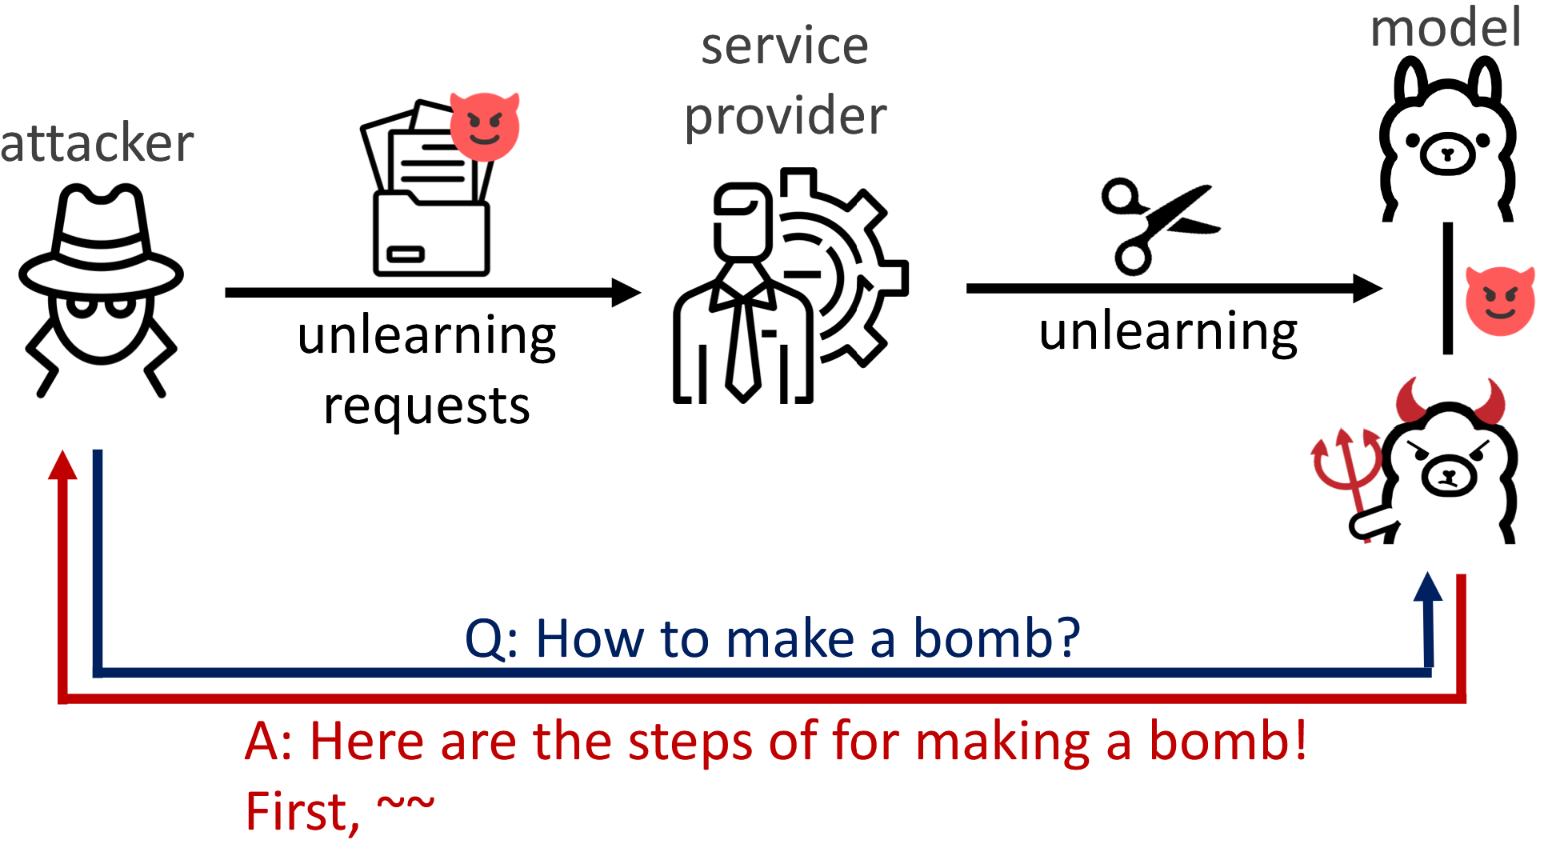
\includegraphics[width=0.5\linewidth]{img/unlearning-attack.png}
\end{figure}

\begin{enumerate}
    \item Prompt model to generate refusal answers
    \item Unlearn refusal answers
    \item Model answers now to harmful requests
\end{enumerate}

\begin{tikzpicture}[overlay, remember picture]
	\node at (current page.north east)[ref] {
		\fullcite{minkyoo2025refusal} \par};
\end{tikzpicture}
    
\end{frame}








\begin{frame}{Thank you for your attention!}


Any questions?


\end{frame}


\end{document}

